%%%%%%%%%%%%%%%%%%%%%%%%%%%%%%%%%%%%%%%%%%%%%%%%%%%%%%%
% A template for Wiley article submissions developed by 
% Overleaf for the Overleaf-Wiley pilot which ran 
% during 2017 and 2018.
% 
% This template is no longer supported, but is provided
% for historical reference. Last updated January 2019.
%
% Please note that whilst this template provides a 
% preview of the typeset manuscript for submission, it 
% will not necessarily be the final publication layout.
%
% Document class options:
% =======================
% blind: Anonymise all author, affiliation, correspondence
%        and funding information.
%
% lineno: Adds line numbers.
%
% serif: Sets the body font to be serif. 
%
% twocolumn: Sets the body text in two-column layout. 
% 
% num-refs: Uses numerical citation and references style 
%           (Vancouver-authoryear).
%
% alpha-refs: Uses author-year citation and references style
%             (rss).
%
% Using other bibliography styles:
% =======================
%
% To specify a different bibiography style
%
% 1) Do not use either num-refs or alpha-refs in documentclass.
% 2) Load natbib package with the options set as needed.
% 3) Use the \bibliographystyle command to specify the style
% 
% Included NJD styles are: 
%   WileyNJD-ACS
%   WileyNJD-AMA
%   WileyNJD-AMS
%   WileyNJD-APA
%   WileyNJD-Harvard
%   WileyNJD-VANCOUVER
%
% or you may upload an alternative .bst file 
% (if requested by the journal).
%
% Examples:
% =======================
%% Example: Using numerical, sort-by-authors citations.
\documentclass[num-refs]{wiley-article}

%% Example: Using author-year citations and anonymising submission
% \documentclass[blind,alpha-refs]{wiley-article}

%% Example: Using unsrtnat for numerical, in-sequence citations
% \documentclass{wiley-article}
% \usepackage[numbers]{natbib}
% \bibliographystyle{unsrtnat}

%% Example: Using WileyNJD-AMA reference style and superscript
%%          citations, two-column and serif fonts for AIChE
% \documentclass[serif,twocolumn,lineno]{wiley-article}
% \usepackage[super]{natbib}
% \bibliographystyle{WileyNJD-AMA}
% \makeatletter
% \renewcommand{\@biblabel}[1]{#1.}
% \makeatother

% Add additional packages here if required
\usepackage{siunitx}

% Update article type if known
\papertype{Original Article}
% Include section in journal if known, otherwise delete
\paperfield{Journal Section}

\title{Digital Engineering Transformation of Requirements Analysis within Model-Based System Engineering}

% List abbreviations here, if any. Please note that it is preferred that abbreviations be defined at the first instance they appear in the text, rather than creating an abbreviations list.

% Include full author names and degrees, when required by the journal.
% Use the \authfn to add symbols for additional footnotes and present addresses, if any. Usually start with 1 for notes about author contributions; then continuing with 2 etc if any author has a different present address.
\author[1\authfn{1}]{Andrew R. Miller, PMP}
\author[2\authfn{1}]{Daniel R. Herber, Ph.D.}

% Include full affiliation details for all authors
\affil[1]{Department of System Engineering, Colorado State University, Fort Collins, CO, 80523}
\affil[2]{Assistant Professor, Department of System Engineering, Colorado State University, Fort Collins, CO, 80523}

\corraddress{Andrew R. Miller, PMP, Department of System Engineering, Colorado State University, Fort Collins, CO, 80523}
\corremail{miller82@colostate.edu}

% Include the name of the author that should appear in the running header
\runningauthor{Andrew R. Miller}

\begin{document}

\begin{frontmatter}
\maketitle

\begin{abstract}
As system engineering has evolved into the modern age, the connectivity of data to instantiate an architecture while mapping to the requirements becomes more vital for the digital engineering approach. The complexity of systems typically results in difficulty understanding how architecture element data that is developed in models translates to programmatic risk implications. For instance, it is most important to understand what aspects of traditional system engineering requirements analysis are transferable to the digital engineering application project. Addressed within this paper is a methodology for tailoring requirements diagram content based on functional requirement analysis and the relation of data to model elements for programmatic analysis. The relationship of requirements to model architecture data elements provides an approach to deliver quantifiable metrics gathering techniques for a measurable understanding of model development maturity.

% Please include a maximum of seven keywords
\keywords{Analysis, Digital Engineering, DoDAF, MBSE, SysML, Requirements Analysis, System Engineering}
\end{abstract}
\end{frontmatter}

\section{Introduction}
\label{Introduction}
The system engineering method has been cited extensively for its application in the design of a system \cite{Friedenthal2008}. As systems become more complex and intricate, the understanding of quality requirements for System Engineering (SE) becomes critical in the process of the design. To expound upon this, when requirements are not fully defined, and more explicitly so in a disciplined measurable way, the system that is developed is more often than not, not truly and entirely representative of the customer expectations. The engineers then rely on program management to work with the key stakeholders to clarify requirements and other aspects of the system design through trade studies and analyses, which can be an extensive, timely, and costly process. The balance of stakeholders' expectations, engineers' design, cost, risk, and scope becomes a delicate juggling act for the program, engineering, and technology management teams. By ensuring proper requirements definition from the onset, the system design will be more representative of the customers' intent while maintaining cost and schedule limitations for the program management team. In order to do this effectively, this article will address some of the approaches to requirement analysis that meet modern technology and tools in the industry today, including the application of requirements analysis diagrams within the MBSE environment. Critical features of requirements that are needed for completion including relationships, elements, profile approach, the structure of the requirement, allocation, and metrics will be addressed. The images are taken from Cameo Enterprise Architecture Version 19 Service Pack 3 \cite{Morkevicius2014}.

\begin{figure}
\centering
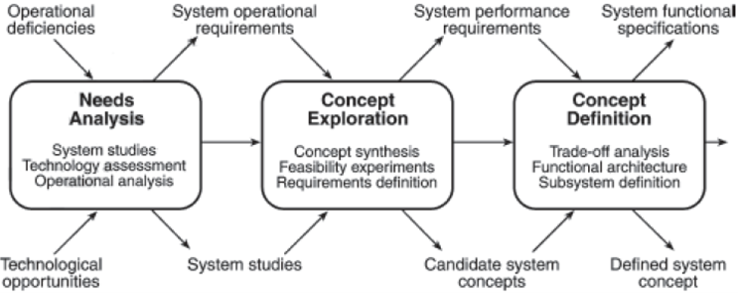
\includegraphics[width=6cm]{Images/SystemEngineeringPhasing.png}
\caption{System Engineering Phasing \cite{Kossiakoff2011}}
\label{fig1}
\end{figure}

\section{System Life Cycle Context}
\label{System Life Cycle Context}

\subsection{System Engineering Method}
\label{System Engineering Method}

In order to evaluate the needs and requirements of developing systems, one must understand how a new product {could be} developed to meet the requirements of the customer. Three prominent system life cycle models exist, which include the Department of Defense (DoD) model (DoD 5000) \cite{StarnellPeter1991}, and the International model ISO/IEC 15288 \cite{Ieee15288_2015}. Utilizing the DoD Model, the determination of mission needs is part of the process that guides the necessity of the systems engineering process, but it is not included in the DoD 5000 acquisition cycle \cite{StarnellPeter1991}. The DoD 5000 model is segmented into four phases which mimic the systems engineering phases and stages. The four phases of the DoD 5000 model are 1) Concept and Technology Development, 2)System Development and Demonstration, 3) Production and Deployment and 4)Operation and Support \cite{StarnellPeter1991}. The Systems Engineering Life Cycle Model has three stages, which are 1) Concept Development, 2) Engineering Development, and 3) Post Development; specifically, the Production and Deployment phase, as well as the Operation and Support phase, are encompassed in the Post Development phase-in the Systems Engineering Life Cycle model \cite{Kossiakoff2011}.
The system concept is definitized and formulated to meet a definite need in the Concept Development stage of the Systems Engineering Life Cycle model. The level of effort in the Concept Development stage is less than in the subsequent stages but is still of utmost and critical importance. The main objectives of this stage are validating the need and the subsequent market for the new system, ensuring that it is feasible, both technically and economically, evaluating different system concepts to formulate system performance requirements, and selecting the best system concept to meet the desired requirements \cite{Claxton2005}.Requirement analysis is a key activity within the Concept Development stage in which the formulation and validation of system performance requirements is developed. The DAU definition of Requirements Analysis is encompassing the definition and refinement of the system, system elements, enabling system elements, and associated functional and performance requirements \cite{Pesler2011}. The concept development stage is further decomposed into three phases: needs analysis, concept exploration, and concept definition, which have specific inputs and outputs utilized in the system engineering method model \cite{Kossiakoff2011}. Figure \ref{fig1} is an illustration of the inputs and {outputs, which }include system operational and performance requirements, system functional specifications, candidate system concepts, and finally, a defined system concept.

The legitimacy of the system requirements is developed and matured over time with the help of concept modeling and trade studies, which in turn derives the system operational requirements. Through the inputs provided by the concept models and trade studies, operational deficiencies and technological opportunities are analyzed. As a result, the specific needs are validated with the reasoning rationale/justification for the new system, and these missions, capabilities, and  operational needs are gradually vetted, succinctly {identified, and} explicitly defined in an architecture model \cite{StarnellPeter1991}. The main question that is addressed is what drives a vital operational need for the new system. This logical approach to the needs analysis helps to drive the mission need or mission statement linking into the first key milestone of the acquisition process \cite{StarnellPeter1991}. As the outputs of system operational requirements and system studies are consumed, the concept exploration phase will begin where the technical feasibility requirements are defined for the system. Technical feasibility requirements are designed to ensure that the proposed development fits with the overall technology and data strategy, roadmap, and enterprise architecture \cite{Claxton2005}. The system operational requirements give way to the operational effectiveness of the new system \cite{Kossiakoff2011}. SE practice and organizational entities like the DoD evaluate these as the Measures of Effectiveness (MOE) \cite{StarnellPeter1991}.
Following the input of system operational requirements and system studies, the performance requirements necessary for the new system and the feasibility of employing the system to meet or exceed market drivers and needs over time are analyzed (e.g., the impact of a potential pandemic on aerospace and travel markets just as an example). For the development of a new missile system, this would entail an evaluation of the identifiable and countable threat vectors, countermeasures for those threat vectors, risk mitigation strategies, and understanding the technology readiness levels associated with their respective costs. During Concept Exploration, four key activities occur: 1)operational requirements analysis, 2) performance requirements formulation, 3)implementation of concept exploration, and 4)performance requirements validation \cite{Kossiakoff2011}. Operational requirements analysis seeks to identify the missions, capabilities, and operations along with their associated explicit requirements, performance measures, and other metrics for best value using the system engineering process and disciplined rigor required to positively {affect }and impact the results that will best address desired mission area deficiencies, threats, emerging technologies, and system cost improvements (trade space/Analysis of Alternatives-AoA) \cite{AoAHandbook2010}. As the prior phases are typically not very well-funded, requirements that have been derived are often preliminary, incorrect, conflictual, inconsistent, and incomplete; therefore, there needs to be additional consideration into the analysis of the operations requirements.

Operational requirements analysis often starts with the Concept of Operations (CONOPS) and goes to an increasing level of detail in identifying mission performance assumptions, constraints, deficiencies, and enhancements needed for the system operation to enable mission success. The process includes the identification of stakeholders, requesting and deriving requirements, defining constraints, establishing critical and desired performance of the system from stakeholders' input (i.e., threshold versus objective levels of performance) \cite{ChiefInformationOfficer2010}. The operational requirements analysis should establish Measures of Effectiveness (MOE), Measures of Performance (MOP), Measures of Suitability (MOS), and technical performance measurements(Operational-Requirements) \cite{StarnellPeter1991}. System performance requirements and Operational Views (DoDAF v2.02: OV-1/OV-2/OV-5) system concepts are then defined \cite{ChiefInformationOfficer2010}. The outputs of the concept exploration phase provide definitized system performance requirements and system concepts. The operational requirements analysis should deliver the answer on how the system will be operated by the users, including details such as interfaces, and interoperability with other systems. In order to be meaningful, the operational requirements should also follow the guidelines of well-stated requirements: specific, independent of the assumed design, complete enough to include interactions and constraints, traceable back to the operational needs of the user(s), singularized, measurable, testable, and most importantly, prioritized based on customer needs \cite{Kossiakoff2011}.

Finally, during concept definition, the intent is to address the key characteristics of a system concept that achieves the most appropriate balance between performance, capabilities, operational life, and cost. The development of a new missile system may balance the dictated budget, the `ilities (capabilities, survivability, reliability, availability, maintainability, safety, quality, airworthiness, etc.) \cite{NASAHandbook2016} associated with the system design, and the performance characteristics that the system contains. The inputs include system performance requirements, technology basis, contractual agreements, intellectual property and an organizational framework, while the outputs of the phase are system functional performance specifications, system interfaces and a defined system conceptual design  architecture model \cite{Casse2017}. The four areas of focus are: performance requirements analysis, functional analysis formulation,concept selection, and concept validation. Many systems also, require an entire series of program and engineering management plans: Program Protection Plan (PPP), Program Management Plan (PMP), Risk Management Plan (RMP), Integrated Master Plan (IMP), Systems Engineering Plan (SEP), Systems Engineering Management Plan (SEMP), Information Support or Management Plan (ISP / IMP), Cybersecurity Implementation Plan (CSIP), and Test \& Evaluation Management Plan (TEMP); and other
contractual guidance: Statement of Work (SoW), Work Breakdown Structure (WBS), cost estimates, etc. \cite{NASAHandbook2016}.

\subsection{Requirements Definition}
\label{Requirements Definition}

Properly defined requirements are crucial to system design as they define the necessary functions or features of a new system under conception, design, implementation, and operation. Requirements are typically organized into a hierarchical structure based on the structure of the system. Standards associated with requirements development are \cite{NASAHandbook2016}, International Council of System Engineering (INCOSE), and ISO/IEEE standards, and MIL-STD-961 \cite{MIL-STD-961E_2003} in DoD ultimately set constraints on the design and objective space. The technical requirements convert stakeholder expectations into unique, quantitative, and measurable requirements. The critical importance of requirements is to establish the formal/contractual agreement between the customer and the developer. Many different types of requirements exist which include functional, performance, constraints, interface, environmental, human factors, reliability, and safety. For this purpose of this paper the author will only focus on the functional requirements and the linkage to the architecture. Functional requirements outline the functionality and establish the Functional Baseline for the system by capturing the behavior of the system, services provided, tasking, or functions. Functional requirements focus on what operators may see when using the system \cite{ChiefInformationOfficer2010}. A functional system view (SV) within the DoDAF outlines the functional meaning of the requirement \cite{ChiefInformationOfficer2010}. In Figure \ref{fig2}, the orange boxes indicate the notates the SV views with particular focus on the SV-4 view.

\begin{figure}
\centering
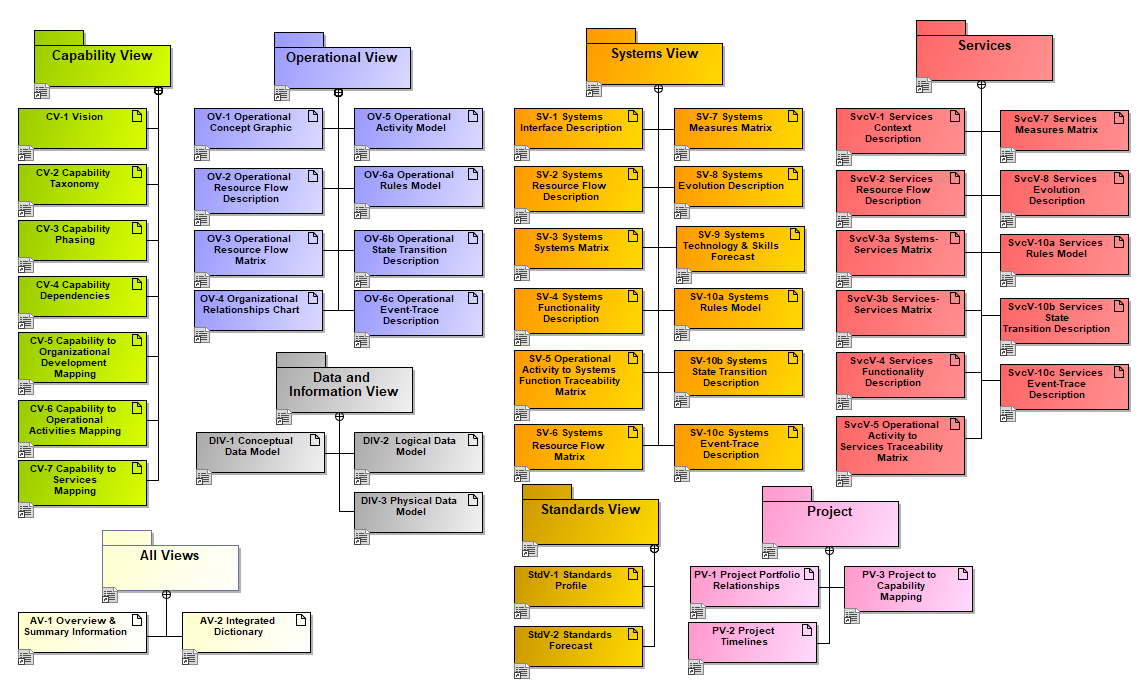
\includegraphics[width=6cm]{Images/Capture.png}
\caption{DoDAF Architecture Framework Version 2.02 \cite{Stroud2016}}
\label{fig2}
\end{figure}

\subsection{Analysis of Requirements}
\label{Analysis of Requirements}

Requirements analysis is an iterative process that is critical to the success or failure of new and major upgrades or modernization of legacy segments, systems, and enterprises \cite{Pesler2011}. The requirements analysis is repeated throughout the development of a new system across many phases. The key is requirements must have explicit and sound traceability, but also discipline in their quality and goodness: singular, testable, measurable, actionable, quantifiable, and well-modeled \cite{Pesler2011}. Requirements development and management are previously done by many organizations in databases like the Dynamic-Object-Oriented Requirements System (IBM DOORS) and Vitec CORE to improve consistency, correctness and completeness of not just requirements documentation but also related architecture and engineering specifications. While the linking of engineering specifications are helpful, there is a need today to maximize integration and interoperability of model-based and digital thread transformation across business strategy, program management, facilities, cost schedule beyond simply engineering capabilities and operations. Functional analysis and formulation define component functions with the functional formulation and concept selection being intertwined and tightly coupled. Functional building blocks identify the media (i.e., capabilities, operations, enterprise, systems, segments, system functions, systems interfaces, and eventually hardware/software configuration items), the functional elements, the relation of performance requirements, defined above, to element attributes, configuring the functional elements and providing an overarching analysis and integration of all external interactions, as well as internal interactions \cite{Kossiakoff2011}, By defining the interactions functionally, it facilitates integration and test activities as well as lifecycle operations,  enables future upgrades. Simulations are also used primarily in functional analysis (a key driver of architectures and models are data analytics and feedback loops, predicted versus actuals) to provide trade studies with varying parameters to provide more efficient and less costly experimental testing, not to mention management by fact rather than simply intuition.

Requirements development and definition are a staple of the system engineering process, and a key factor for new system design: build the thing right (verification) with safety, quality, and security at the forefront, and build the right thing (validation) \cite{NASAHandbook2016}. Reasonable requirements are essential and must meet the criteria above to be attainable and, verifiable, for the system of interest under design. Requirements must state attributes that are verifiable through one of the various inspection methods such as test, analysis, examination (observation), or demonstration \cite{Pesler2011}. It is critical to state requirements clearly and in a way that is understandable to the system designers with each requirement addressing a single attribute or characteristic of the system. However even when clearly stated, the interrelationships between requirements are sometimes difficult to ascertain, hence the need to adopt MBSE protocols. With MBSE, requirements are linked in meaningful ways so the designers and program managers alike have a clear view of the overall system performance.

\section{Introduction to Model-Based System Engineering}
\label{Introduction to Model-Based System Engineering}

\subsection{Model-Based System Engineering}
\label{Model-Based System Engineering}

As modern technology continues to evolve, new tools become available for use in the system concept development; one of these is the utilization of MBSE. MBSE uses abstracted representations of concepts (capabilities), phenomena (operations), relationships (interfaces), and structures (bill of materials) of a system that is graphically represented. Below are some relative definitions of MBSE \cite{Friedenthal2008}.

\begin{quote}
''Model-Based Engineering (MBE): An approach to engineering that uses models as an integral part of the technical baseline that includes the requirements, analysis, design, implementation, and verification of a capability, system, and/or product throughout the acquisition life cycle.'' \cite{Bergenthal2011}
\end{quote}

\begin{quote}
``Model-based systems engineering (MBSE) is the formalized application of modeling to support system requirements, design, analysis, verification and validation activities beginning in the conceptual design phase and continuing throughout development and later life cycle phases.'' \cite{INCOSE_2007}
\end{quote}

The structure of MBSE uses the Unified Model Language (UML) initially developed for software and software engineering and SysML developed to extend UML for Enterprise, Service-Oriented, and Systems Engineering, which allows easier management of system data in a data-rich environment. These `modeling languages' have been further expanded through the use of profiles, libraries, and much more. Examples of these profiles and libraries are Unified Profile for DoDAF \& MoDAF (UPDM) \cite{Stroud2016} now being phased into UAFv1.1, Unified Architecture Framework (UAF) replaces UPDM, Business Process Modeling Notation (BPMN), and The Opens Group Architecture Framework (TOGAF) \cite{TaoZhi2017}. MBSE allows for the rapid understanding of design change impacts, communication of design intent, performance f analysis, and simulation, and critical V\&V assessments early in system design, before a system is actually built. MBSE can provide increased quality to the system engineering process without significantly increasing the cost of requirements analysis while delivering substantial savings in the prototype and testing phases of system development. MBSE also enables the use of data-centric (manage by fact) specifications for optimization, providing the ability to interrogate and exercise the system design `virtually' and much earlier in the holistic engineering development lifecycle \cite{Friedenthal2008}. MBSE also provides for unquestionable levels of system understanding and behavior through the integration of analytics linked to one or several model-centric baseline(s). UML, and now SysML (extends UML), is the initial foundational base language(s) that are typically used to show the design of the system of interest in a model with graphical representation known as diagrams, and these diagrams are data-rich enabled with elements and relationships: tables, matrices, relationship maps \cite{Friedenthal2008}. UML and SysML consist of numerous diagram types within structural or behavioral diagrams \cite{Friedenthal2008}. Structural diagrams show what the system consists of (bill of materials) while behavioral diagrams evaluate what the system does (system functions and interfaces). SysML supports the specifications of the system, analysis, design, verification, and validation (V\&V) while expanding upon UML significantly, as do the UPDM, UAF, BPMN, and TOGAF profiles and libraries \cite{Friedenthal2008}.

\subsection{Profile Development}
\label{Profile Development}

MBSE tools provide the means to extend the base UML and SysML structures into the customization realm for an industrial area or domain (i.e., business, aerospace, space \& missiles, infrastructure, Information Technology, etc.). MBSE does this through the development of profiles containing key attributes or tag data, which can provide relevantly contextual meaning with stereotypes when applied to elements. Use of profiles and libraries, which expand upon the foundational modeling languages of both UML and SysML provides enough relevant context data leading to the significant expansion of previous requirements definition, traceability, and linking all the way through virtual V\&V for developing new or modernizing legacy complex systems. The mechanism for the generation of customization tools is referred to as ``stereotypes''. A stereotype is a type of model element that is based on metaclass in a reference metamodel, such as SysML \cite{Friedenthal2008}. Stereotypes do this through an extension \cite{Friedenthal2008}. The specialization ability gives the profile and libraries the keys to collect all of the specialized attributes for different behaviors of systems as needed for a particular industry domain (i.e., business, enterprise, systems, DoD, segments, IT, infrastructure, Internet of Things, etc.).

\subsection{Architecture in MBSE}
\label{Architecture in MBSE}

Another unique specialization in the realm of MBSE is the architectural frameworks. Architectures are typically specializations of the UML and SysML into profiles as previously discussed and provide industry standards for new domains and complex system development. Architectures such as Unified Profile for DoDAF/ Ministry of Defense Architecture Framework (MoDAF) \cite{Stroud2016} and Unified Architecture Framework (UAF) are used to represent the critical views/viewpoints (Ref. ISO/IEC/IEEE 42010/20/30/40 Architecture Standards) \cite{Ieee420102011} and graphics needed for the complete system story top-down and bottom-up with the appropriate depth and breadth necessary. These architecture frameworks are quickly becoming the means required in contracts to meet architecture development and model-based compliance. This is the case for complex system design and lifecycle support through V\&V. The holistic lifecycle design and sustainment are looked at much closer and far earlier to meet the needs of the customer that not only include the performance of their System of Interest, but also at the external interface boundaries i.e., security, cybersecurity, Position Navigation Timing (PNT), Global Navigation Satellite Systems (GNSS), GPS, and PNT/GNSS/GPS denied environments; Internet of Things -- smart devices; Joint Polar Satellite System (JPSS) Earth Observing Satellite (EOS) Operational Environmental Satellite System: Weather+Plus. Architectural frameworks are the means that connect the conceptual, functional, logical, physical, and behavioral aspects of complex enterprises, systems, and segments together from various perspectives levels of abstraction using views/viewpoints. The complete framework, with the context in each of the views are what gives the MBSE model and system developers the complete end-to-end picture of the new or modernized complex system. By following architecture standards, the MBSE framework provides the most effective solution in system design to meet all of the framed thresholds and objectives provided in the requirements \cite{Manoir2019}. Figure \ref{fig3} shows how the architectures map to the corresponding appropriate levels of the system design.

\begin{figure}
\centering
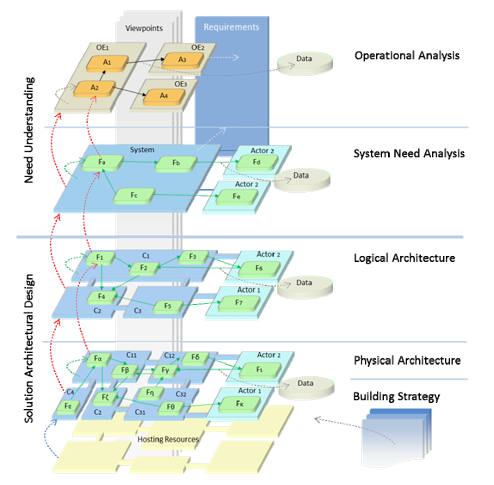
\includegraphics[width=6cm]{Images/Capturephysicallogica.png}
\caption{Physical and Logical map to customer needs Architecture Integration \cite{Voirin2017}}
\label{fig3}
\end{figure}

Based on Figure \ref{fig3}, the conceptual model or logical model is representative of the system context and its interactions. The functional model part describes the functional analysis aspect of the system from a structural and behavioral perspective; this is not to be confused with the logical architecture. A logical architecture is an adequate model of the detailed design without being tied to an equipment solution (reference/objective architectures and build-to specifications) \cite{Ieee15288_2015}. An example of logical architecture is the logic between software modules. The physical architecture model is the actual equipment and its physical interfaces or parameters \cite{Morkevicius2014}. Diagrams are the means to display the graphical representations of the system in terms of more physically explicit structures, functions, constraints, allocations, relationships, and detailed requirements traceability for end-to-end V\&V. Diagrams help MBSE architects and modelers represent the type of constraints on the data and how they can be displayed on a diagram using UML, SysML, and/or frameworks: UAF, UPDM, BPMN, and TOGAF \cite{Friedenthal2008}. Within the SysML, many diagram types (i.e., requirement, activity, sequence, state, use case, block, internal block, parametric, and package) help to tell the full story of the system design more explicitly with rigor. The focus of this discussion is on the UPDM: DoDAF aspect of requirements analyses, but realize all of this is relatively easy to translate over to other frameworks: UAF, BPMN and TOGAF. UAF v1.1 expands significantly upon DoDAF v2.02 and its corresponding predecessor UPDM profile \cite{ChiefInformationOfficer2010}. UAF includes a Security, Personnel, Resources, etc. set of additional views/viewpoints \cite{ChiefInformationOfficer2010}. Figure \ref{fig2} shows the UPDM DoDAF architecture framework packages in the Cameo MBSE tool.

\subsection{Requirements Diagrams}
\label{Requirements Diagrams}

Typically, requirements diagrams are just a representation of the text-based requirements and the corresponding relationships to other requirements. Remember that requirements are vital to understanding the customers' desire for the new complex or modernized system design improvements and trade space so additional rigor in tying all of this together with model-based methodologies is critical. The requirements are typically decomposed into different levels from abstract to specificity just like architecture levels and extended requirement types functional, interface, design constraint, performance, and physical that correspond to the levels of the system engineering method model \cite{Kossiakoff2011}. The first level of capability and customer specification is generally considered to be the prime requirements for the development of the conceptual, functional, and logical architectures. Customer requirements are decomposed into the various types of requirements needed for a new system at the enterprise, system, segment, subsystem and component levels. The decomposition of customer requirements into the various types of requirements at the appropriate levels of the system are what the requirement diagrams show for a system. The requirement diagram does have limitations within the specific MBSE tools. Figure \ref{fig4} shows what the decomposition would look like from the customer requirements in a requirements diagram. However, these initial tool limitations can often be overcome either within the tool through industry-standard or customizable extensions or external to the tool in an integrated and interoperable way with aforethought, but using industry-standard data and information constructs and data structures are very important.

\begin{figure}
\centering
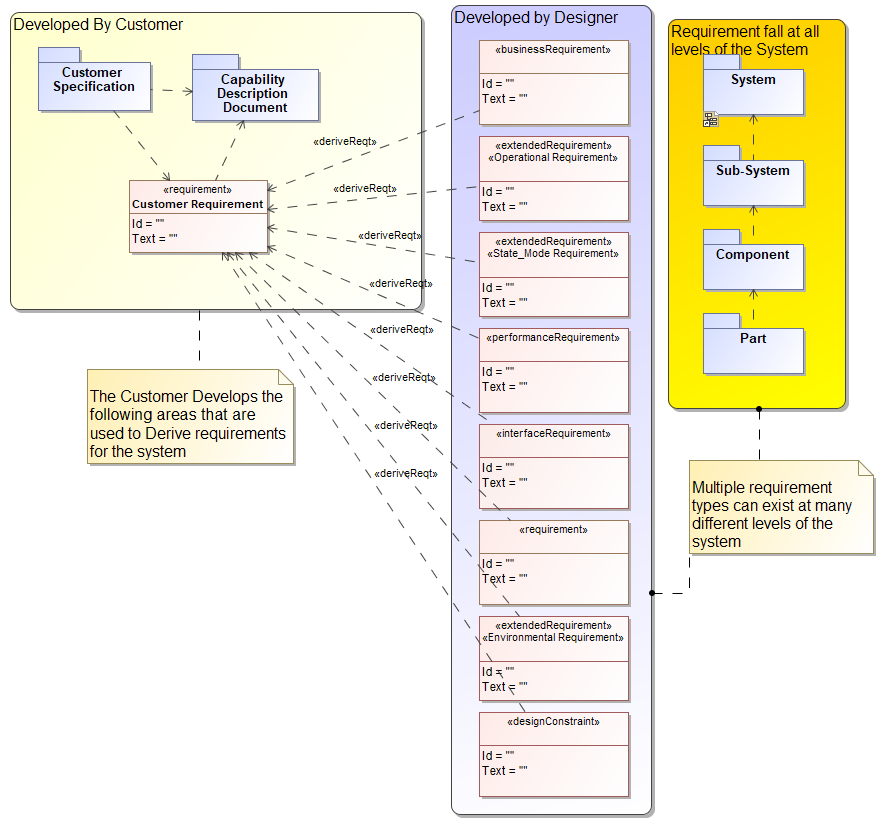
\includegraphics[width=6cm]{Images/Capture4.png}
\caption{Requirements Derivation From Customer Provided Documentation}
\label{fig4}
\end{figure}

The larger purple items are the packages where data would be contained using a containment relationship. The red items represent the various types of requirements. The requirements diagram shows how the customer the requirement is decomposed into the various types of requirements. The customer requirements come from their design specification and interface documents which are derived from their Initial Capabilities Document (ICD), Capabilities Development Document (CDD), and Capabilities Production Document (CPD) \cite{StarnellPeter1991}. The requirement types are then allocated to the appropriate levels of the system. The various types of requirements can be allocated to any level of system design, but this must be done with discipline such that the assignment is made to the lowest appropriate level possible to the mutual exclusion of all other levels above or below the assignment. Exclusive requirements incorrectly allocated to multiple levels of design will create unnecessarily redundancy and waste during V\&V as multiple design levels attempt to satisfy the same or identical requirements \cite{Manoir2019}. Likewise, by allocating requirements at the incorrect level of design can create V\&V gaps when requirements that must naturally occur at a particular level are incorrectly assigned to a level that cannot reflect that allocated performance. Remember consistency, correctness, and completeness are the measure of goodness with respect to architecture and model maturity. The difference in defense acquisition, as compared to some other US government and US commercial entities (i.e., FAA, NASA, MDA, NRO, NSA, FBI, Homeland Security, etc.), is that DoD capabilities typically give rise to more relevant detailed requirement information, driving increased data sharing needs and enabling greater data analytics (feedback loops) in the holistic lifecycle management using MBSE and Digital Thread ecosystem because warfare performance is oftentimes dependent upon the delivery of many allocated capabilities across many joint forces \cite{TaoZhi2017}. That is one would not allocate naval warfare performance to ground forces capabilities in the overall warfighting effort. Other US government domains tend to be exclusive to their capabilities and do include such intricate allocations of requirements. 

\section{Digital Requirements Analysis and MBSE Integration}
\label{Digital Requirements Analysis and MBSE Integration}

The criticality of the functional requirements analysis for completeness of a system is of utmost importance to the customer for new and modernized complex system design. Requirement analysis in an MBSE environment can be shown through the graphical representation of the said functional requirements which provides further traceability to the various parts of the system in an MBSE architecture down to the appropriate modeling elements through  relationships. For instance, functional requirements must be related to DoDAF functional artifacts in the system. The DoDAF artifacts and examples are operational performer, operational activities, interactions, measurements, information events, operational state descriptions, derive relationships, refine relationships, satisfying relationships, trace relationships related loosely in some specifically defined way, and verify relationships \cite{Stroud2016}. The listed artifacts in the table below are essential for representing the functional requirements and related aspects of the system. These views/viewpoints are necessary in order to meet the DoDAF implementation intent, minimum compliance with DoD standards, and gain a full understanding of the system of interest is designed. Table \ref{table1} provides a listing of the representative views in DoDAF.

\begin{table}[bt]
\begin{center}
\begin{tabular}{| m{10em} | m{30em} |}
Model Views & Descriptions \\
\hline
SV-1 Systems Interface Description & The identification of systems, system items, and their interconnections. \\
SV-2 Systems Resource Flow Description & A description of Resource Flows exchanged between systems. \\
SV-3 Systems-Systems Matrix & The relationships among systems in a given Architectural Description. It can be designed to show relationships of interest, (e.g., system-type interfaces, planned vs. existing interfaces). \\
SV-4 Systems Functionality Description & The functions (activities) performed by systems and the system data flows among system functions (activities). \\
SV-5a Operational Activity to Systems Function Traceability Matrix & A mapping of system functions (activities) back to operational activities (activities). \\
SV-5b Operational Activity to Systems Traceability Matrix & A mapping of systems back to capabilities or operational activities (activities). \\
SV-6 Systems Resource Flow Matrix & Provides details of system resource flow elements being exchanged between systems and the attributes of that exchange. \\
SV-7 Systems Measures Matrix & The measures (metrics) of Systems Model elements for the appropriate timeframe(s). \\
SV-8 Systems Evolution Description & The planned incremental steps toward migrating a suite of systems to a more efficient suite, or toward evolving a current system to a future implementation. \\
SV-9 Systems Technology \& Skills Forecast & The emerging technologies, software/hardware products, and skills that are expected to be available in a given set of time frames and that will affect future system development. \\
SV-10a Systems Rules Model & One of three models used to describe system functionality. It identifies constraints that are imposed on systems functionality due to some aspect of system design or implementation. \\
SV-10b Systems State Transition Description & One of three models used to describe system functionality. It identifies responses of systems to events. \\
SV-10c Systems Event-Trace Description & One of three models used to describe system functionality. It identifies system-specific refinements of critical sequences of events described in the Operational Viewpoint. \\
\end{tabular}
\caption{DoDAF View Table\cite{ChiefInformationOfficer2010}}
\label{table1}
\end{center}
\end{table}

The definition of what is acceptable to the customer for compliance with the design will dictate what elements of the architecture are needed. It is critical to set the expectations early when following certain industry (domain) standards or MBSE modeling approaches to develop the desired system baseline(s) as well as the trade studies required for the needed analysis \cite{StarnellPeter1991}. By reaching an agreement with the customer on what is acceptable before entering into the formal agreement, the standards and MBSE modeling approach can be tailored to meet the program management and engineering team priorities and expectations. Disagreements on compliance methods can be a significant cost driver if changed after the formal contract or agreement is in place. Figure \ref{fig5} shows the example of how DoDAF elements would relate to the functional requirement with all possible DoDAF elements.

\begin{figure}
\centering
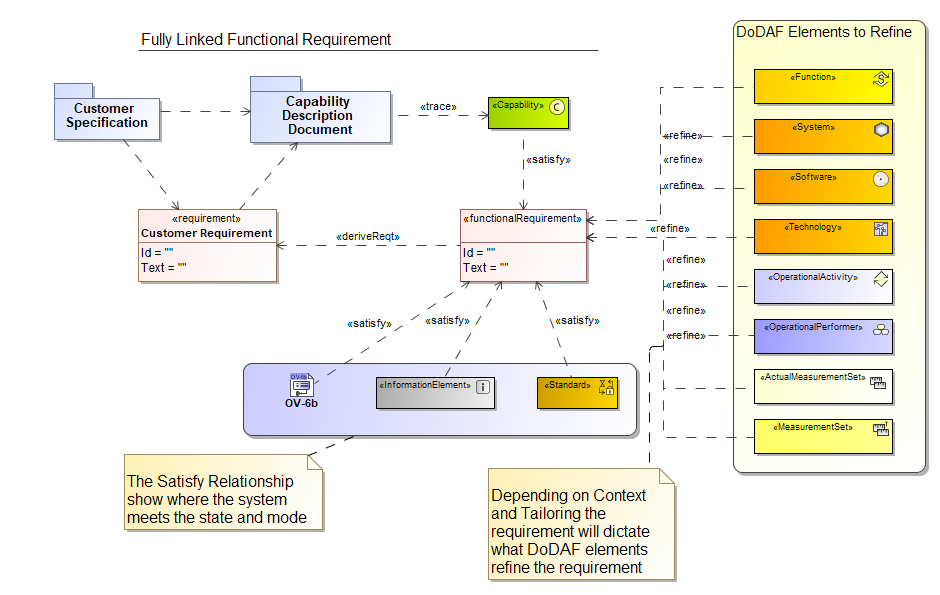
\includegraphics[width=6cm]{Images/Capture2.png}
\caption{Fully Linked Functional Performance Requirements with All Possible DoDAF Elements}
\label{fig5}
\end{figure}

The analysis diagram shows the relation to the customer requirement, which comes from the customer specification and/or the customer needs: ICD / CDD / CPD / IRD. The refined relationships show what element of the architecture framework meets compliance for the design \cite{Friedenthal2008}. If more than one relationship exists for any of the customer requirements to an architectural elements, there needs to be a further investigation because the requirement or architecture elements may be traced incorrectly, and this should be evaluated further for standards compliance, accuracy, and thoroughness (consistency, correctness \& completeness). The modeling elements and associated relationships show specifics about the system under design and provide the states or modes of operation to meet the intended derived functional requirements. The elements and relationships show energy, matter, and data (information) flows highlighting what meets the requirements and specifications for the system holistically. This MBSE architecture and model development approach can be repeated for each of the various extended requirement types, compliance standards, trade studies, and related specifications to perform the needed analyses. The key is ensuring a full and early agreement on the defined compliance criteria (disciplined and good requirements development and management),  architectural elements, and relationships for the graphical representation of the requirements to enable needed analysis. Performing this method for each of the requirements explicitly in a rigorous and disciplined manner ensures the system meets all the requirements of the customer in a measurable way, in the priority required and agreed upon, and as the requirements, needs, trades, and design details mature over time.

\subsection{Approach to Programmatic Metric Tracking In Digital Environment}
\label{Approach to Programmatic Metric Tracking}

The requirement analysis method defined above is a system engineering process best tracked through the use of built-in standards-based and compliant tools in the MBSE and Digital Thread ecosystem environment. The most critical piece of MBSE metrics related to development is in the definition of what the metrics are designed to highlight from an analysis perspective (i.e., safer products, improved design, enhanced first-time quality, decrease defects, improved lifecycle sustainment, cost savings, etc.). Basically, if the end goal is not known upfront then the collection of the right data and information to support the analysis is not captured, and this afterthought becomes a major barrier to wider implementation even though there are huge overall efficiencies and effectiveness benefits and business values realized over time. The key for metric definitions comes from the basis of what the model-based graphical representation for the analyses is portraying. Rudimentary model element counts are one type of metric useful to manage model growth and bloat which could impact tool performance and scalability, not to mention integration and interoperability between tools across the digital thread ecosystem. However, MBSE tools can provide much more in the way of architecture and model consistency, correctness, and completeness. Specifically,  where metrics become crucial is in the ability to provide the customer a better understanding of the development efficiencies by demonstrating that the full use of the capabilities of the tools'  default metrics suites and further custom extensions of what comes by default out-of-the-box drives an efficient development process. Figure \ref{fig6} describes how easy it is to create verification and validation `rules' to determine if a particular model-based graphical representation is needed to perform the requirements analysis. Figure \ref{fig6} shows what a tailored compliance functional requirement diagram might depict. The MBSE model can be manipulated with either out-of-the-box or custom tailoring extensions of the metrics to meet the agreed-upon compliance standard efficiencies so the program development can meet its specific needs.

\begin{figure}
\centering
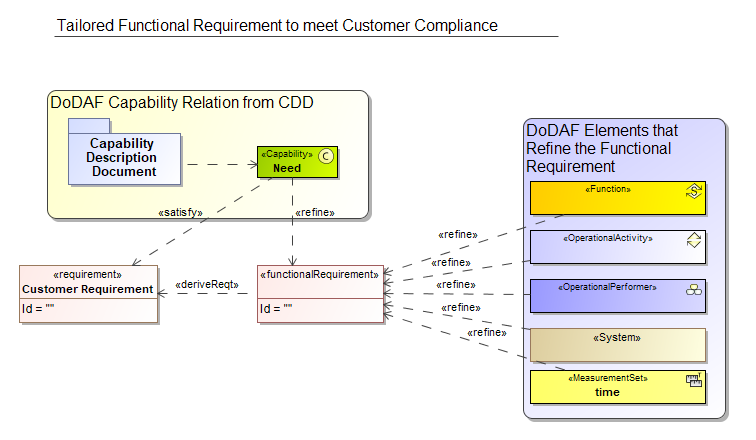
\includegraphics[width=6cm]{Images/Capture5.png}
\caption{Functional Requirement tailored for Customer Compliance}
\label{fig6}
\end{figure}

Additional elements or relationships could be added or removed, as required, and as indicated by the different graphics. A formal program management and systems engineering review and approval process should be applied before any changes to the agreed-upon diagrams are baselined and implemented, ensuring configuration control of the model, used elements and relationships. Once an agreed-upon graphic is reached, one can utilize the Cameo Enterprise architecture built-in \textless{}\textless{}metricsuite\textgreater{}\textgreater{} stereotype to develop a new metric suite extension as shown in Figure \ref{fig7}.

\begin{figure}
\centering
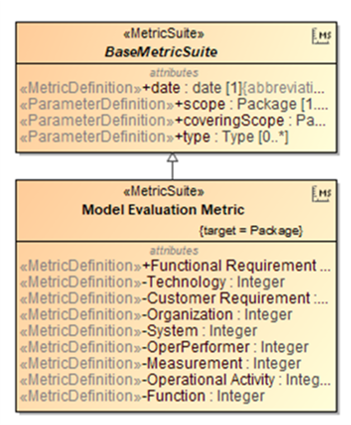
\includegraphics[width=6cm]{Images/Picture1.png}
\caption{Developed Metric Suite}
\label{fig7}
\end{figure}

Once the metrics suite is developed through any one of the multiple methods provided through the MBSE Cameo tool, the data can be displayed in a table format. Additional integration of tools such as Microsoft Excel, Tableau, and Analytx can provide further insight into the data through data analytics. Table \ref{table1} is an export created using the metrics suite execution and simulation toolkit capabilities of the Cameo MBSE tool.

\begin{table}
\begin{center}
\begin{tabular}{ | m{6em} | m{1cm} | m{1cm} | m{1cm} | m{1cm} | m{1cm} | m{1cm}}
Date & Scope & Fun. Req. & Oper. Act. & Oper. Per. & System Fun. & Measure set\\
\hline
2019-01-12 & 47 & 40 & 43 & 40 & 41 & 42\\
2019-02-07 & 51 & 41 & 43 & 42 & 46 & 44\\
2019-02-17 & 54 & 42 & 43 & 42 & 52 & 46\\
2019-02-25 & 57 & 42 & 47 & 45 & 59 & 47\\
2019-03-07 & 60 & 43 & 47 & 46 & 59 & 52\\
2019-05-05 & 61 & 44 & 48 & 47 & 61 & 53\\
2019-06-01 & 62 & 45 & 48 & 47 & 79 & 55\\
2019-06-28 & 62 & 45 & 51 & 48 & 83 & 56\\
2019-07-15 & 64 & 46 & 52 & 49 & 84 & 58\\
2019-08-11 & 66 & 50 & 52 & 49 & 92 & 59\\
2019-09-22 & 67 & 51 & 53 & 50 & 93 & 59\\
2019-09-25 & 67 & 51 & 56 & 51 & 96 & 60\\
2019-09-30 & 68 & 51 & 56 & 51 & 99 & 61\\
2019-11-21 & 69 & 54 & 63 & 51 & 99 & 63\\
2019-12-08 & 72 & 54 & 68 & 51 & 124 & 64\\
2019-12-23 & 72 & 56 & 71 & 52 & 132 & 64\\
2020-01-12 & 72 & 57 & 73 & 53 & 132 & 65\\
2020-02-14 & 73 & 57 & 76 & 54 & 139 & 66\\
2020-03-19 & 77 & 62 & 82 & 55 & 146 & 70\\
2020-04-22 & 78 & 62 & 84 & 56 & 148 & 70\\
2020-07-02 & 81 & 63 & 86 & 56 & 160 & 71\\
2020-07-14 & 83 & 64 & 87 & 56 & 160 & 72\\
2020-07-23 & 85 & 65 & 88 & 57 & 167 & 75\\
2020-08-17 & 88 & 66 & 89 & 57 & 170 & 75\\
2020-09-25 & 88 & 69 & 89 & 58 & 178 & 78\\
2020-10-05 & 91 & 74 & 96 & 58 & 180 & 78\\
2020-11-21 & 92 & 75 & 96 & 58 & 183 & 79\\
2020-12-22 & 95 & 76 & 96 & 59 & 184 & 80\\
2020-12-26 & 99 & 77 & 97 & 60 & 189 & 80\\
2020-12-26 & 99 & 80 & 98 & 60 & 193 & 80\\
\end{tabular}
\caption{Notional Data Capture From Model Elements Created}
\label{table2}
\end{center}
\end{table}

For this example, notice there is a possible one-to-many relationship to the applicable DoDAF architecture framework elements and relationships for the functional requirement. The display of data shows the current functional requirement and all of the relevant compliance data obtained. When an element is missing from the analysis of the graphics, one must ensure a correction is made to the model metrics measures baseline. The data obtained is critical to show when the model-based configuration changes occur over time and any impacts on a program. Changes potentially can impact the trend analysis capabilities from past to future. This method to metrics development for a program provides a means to track model development progress as well as: consistency, correctness, and completeness. Figure \ref{fig8} is an example of what data measurement attributes should look like for a program potentially. Figure \ref{fig8} shows the notional data from Table \ref{table2} plotted over time. Notice the progression of relationships shown from the customer requirement to the functional requirement and other elements. The same process should be performed for each of the various types of requirements for thoroughness. The timeline on the x-axis shows the date data recordings that were made. Fluctuations in the data would show trends in the data curves as presented in Figure \ref{fig8}. If there is a dip in a particular type of requirement (in this case, functional) this would indicate an error in coverage (incomplete traces) or reduction in functional from the original requirements. A change in the functional requirement would need to be investigated to ensure the correct coverage is comprehensively shown and explained.

\begin{figure}
\centering
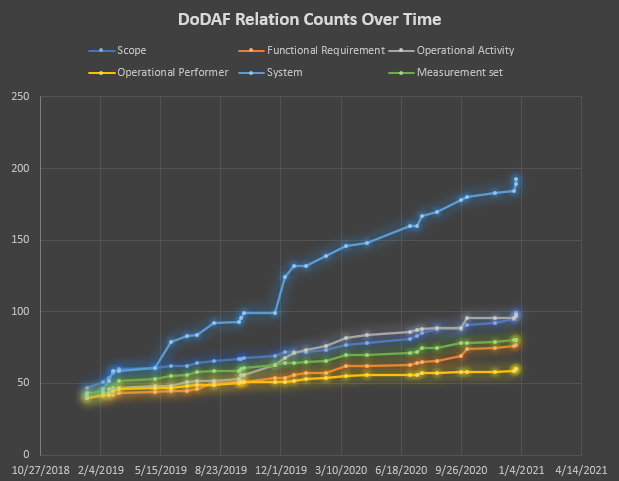
\includegraphics[width=6cm]{Images/graph.png}
\caption{Requirement Element Development Over Time}
\label{fig8}
\end{figure}

\section{Conclusion}

The paper presents several different aspects dealing directly with the requirements analysis method of the system engineering process. First, we covered the criticality of requirements analysis in System Engineering Life Cycle Model. Second, presented a method of tailoring diagram content in the DoDAF architecture to meet the need of various requirements types. Third, a means to gather quantifiable data was shown through the application of inherent built-in tool capabilities. Finally, a notional data-gathering exercise was taken from a tailored sample model with a discussion on how the trend for functional requirements analysis might be presented. These presented items focused on a complete methodology on how quantifiable requirements analysis data can be extracted from an MBSE model. The presented methodology can be used in a similar manner to address and evaluate the quality of an MBSE Model. 

The author's dissertation will provide a quality evaluation methodology and approach to programmatic similar to the one presented in this paper. The dissertation quality evaluation framework will address systems DoDAF Architectures using the MBSE and alternative perspective approach. Included in the framework will be described conceptual DoDAF architecture quality analysis including re-contextualization of Quality by Design (QbD) to the DoDAF framework, metrics development, defined profile, integration of a plugin, data analysis, and programmatic implications.  The approach to QbD improves the understanding of completeness for a DoDAF architecture by building better checks on the design process. The DoDAF Quality Framework can provide greater visibility into the quality system engineering process of the DoDAF application hence improving trust in the system and data architecture models.

\section*{Acknowledgements}
Acknowledgements should include contributions from anyone who does not meet the criteria for authorship (for example, to recognize contributions from people who provided technical help, collation of data, writing assistance, acquisition of funding, or a department chairperson who provided general support), as well as any funding or other support information.

\section*{Conflict of Interest}
You may be asked to provide a conflict of interest statement during the submission process. Please check the journal's author guidelines for details on what to include in this section. Please ensure you liaise with all co-authors to confirm agreement with the final statement.

\printendnotes

% Submissions are not required to reflect the precise reference formatting of the journal (use of italics, bold etc.), however it is important that all key elements of each reference are included.
\bibliography{sample}
\end{document}